\toclesssection{SCP 036 - The Reincarnation Pilgrimage of the Yazidi (Kiras Guhor\^{i}n)}
\addcontentsline{toc}{section}{SCP 036 - The Reincarnation Pilgrimage of the Yazidi}

\textbf{Item \#:} SCP-036

\textbf{Object Class:} Safe

\begin{figure}[h]
\begin{center}
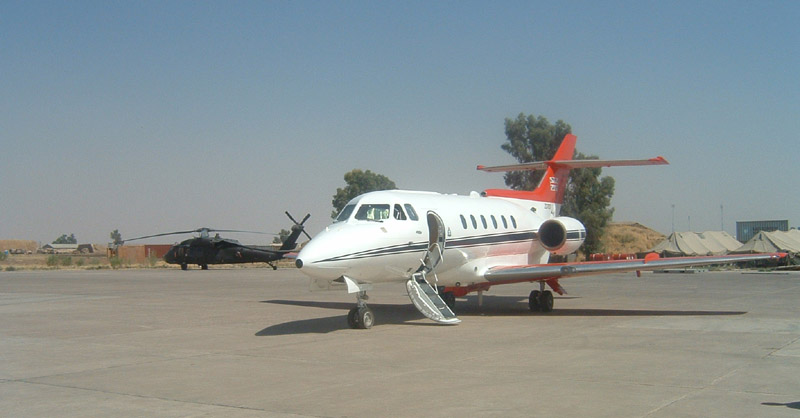
\includegraphics[scale=0.3]{scp/036a.jpg}
\linebreak The Pilgrimage Flight awaiting take-off
\end{center}
\end{figure}

\textbf{Special Containment Procedures:} Once every year, a mobile task force is dispatched from Containment Command-02 in [EXPUNGED] to Site-22A to defend the runway and airport located there. The civilian facility is to be cleared of all non-SCP personnel by 0400 hours of September 23 and none are allowed to return until sunrise the next day. On October 1, all civilians must be evacuated again before sunrise and will not be allowed on to Site-22A until the return of the "Pilgrimage flight."

Pilgrims in transit from the "Arrival Flight" awaiting departure on the "Pilgrim Flight" may only be cross-examined by researchers with Level 3 security level clearance or higher.

\textbf{Description:} SCP-036 includes the location, Site-22A (a small airport in the Mosul region of northern Iraq) and Site-22B (the destination of passengers boarding at Site-22A). The key components of SCP-036 are:
\begin{itemize}
\item The "Arrival flight"- A passenger plane (that varies in make and model from year to year) that arrives shortly before dawn on September 23. It appears on radar about 30-40 kilometers away from Site-22A. When it lands, "pilgrims" exit the plane and enter the terminal. No crew have ever left the plane. Observations have only revealed a masked pilot and co-pilot. This plane leaves quickly after pilgrims exit and does not wait for clearance for take off, nor does it identify itself upon approach for landing.
The "Pilgrims"- People of the Yazidi faith that exit the "Arrival" plane, who are said to be undergoing the ''kiras guhor\^{i}n''. Each year they are examined and identified as various people of the Yazidi faith that have died during the previous year. This is done through birth certificates, photo IDs, specific knowledge questions, and when possible, finger printing. Most have been known to be friendly and amicable though most are reluctant to give details about the kiras guhor\^{i}n. In the past, all have shown to be unable to recognize family and friends or been able to remember any information beyond what short term memory would normally allow. In the late afternoon of September 23rd, most pilgrims begin to emphasize how important it is that their pilgrimage must begin. At that time, they file onto the "Pilgrimage flight" plane and depart, never to be seen again.
\item The "Pilgrimage Flight"- A passenger plane provided by SCP personnel for the transport of "the pilgrims," it is manned by a crew of trained Yazidi holy men. The crew are typically never able to elaborate upon details of the pilgrimage or what the kiras guhor\^{i}n actually is. SCP equipment on board function optimally but recorded data will only slightly increase our understanding of the pilgrimage each year. Though the flight is gone for seven days, the crew and recorded data are only able to account for a few hours. Days are missing from time recording equipment and cameras, though nothing abnormal is ever observed. The plane disappears from radar and visual contact is lost about 50-60 km away from Site-22A until it returns about sunrise on October 1.
\item Site -22B- The destination of the "Pilgrimage plane," it is a small airport consisting of a runway and single building located at coordinates [EXPUNGED]. It has only been observed by "Pilgrimage crew" and cameras on the plane. It does not appear on satellite images and attempts to reach it on foot have failed, once with disastrous results. Cameras have trouble focusing on the area, as the heat from the ground usually causes a mirage-like visual effect on all objects more than a few dozen meters from the plane. A fly over with an SCP reconnaissance plane several weeks before the pilgrimage revealed undeveloped land and and what looked like an ancient stone statue. In the 1990s, SCP Mobile Task Force Sigma-4 attempted to reach Site-22B during the time of the pilgrimage. Upon the approach, communication was lost and the Task force was never heard from again. No other exploration attempts are advised during the seven (7) day pilgrimage.
\end{itemize}
\begin{figure}[h]
\begin{center}
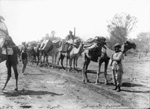
\includegraphics[scale=1.2]{scp/036b.jpg}
\linebreak Yazidi Holy men shortly before the pilgrimage
\end{center}
\end{figure}

Originally, the Kurdish speaking Yazidi people around Mosul secretly performed the Pilgrimage themselves. Pilgrims from the east were escorted by masked armed guards on camel back into the care of Yazidi holy men. It has been explained that the holy men would then take the pilgrims west to their "land of the dead," where the pilgrims would wait to be "reborn" back into the Yazidi people. The ''kiras guhor\^{i}n'', literally Kurdish for "changing garments," is used to describe the belief of reincarnation that lesser souls of the Yazidi undergo. While this actual pilgrimage was done in secret, a symbolic pilgrimage and ''kiras guhor\^{i}n'' are performed every year at this time by other Yazidi.
During the 1960s, land acquisition by Kurds and Muslims, attacks by Turks, and punitive laws by the Islamic Iraqi Government, restricted the movements and customs of the Yazidi. During that time, the Foundation stepped in and offered aid in the way of an advantageous clause that granted SCP planes unrestricted access to airport facilities in the area. Almost immediately, mysterious planes carrying pilgrims from the east began landing at the local airport and an elusive airport at the destination appeared as well.